\documentclass[12pt,a4paper]{article}

% ─── 1. PACKAGES ──────────────────────────────────────────────────────────────
\usepackage[utf8]{inputenc}
\usepackage[T1]{fontenc}
\usepackage{amsmath, amssymb}
\usepackage{geometry}
\usepackage{graphicx}
\usepackage{xcolor}
\usepackage{listings}
\usepackage{hyperref}
\usepackage{booktabs}
\usepackage{enumitem}
\usepackage{tcolorbox}
\usepackage{mdframed}
\usepackage{fancyhdr}
\usepackage{titlesec}
\usepackage{tikz} % Untuk menggambar diagram state Automata
\usetikzlibrary{automata, positioning, arrows.meta}

% Font Settings
\usepackage{newtxtext,newtxmath} % Times New Roman
\usepackage{courier}             % Courier New untuk kode

\geometry{margin=2.5cm}

% ─── 2. WARNA TEMA ────────────────────────────────────────────────────────────
\definecolor{codebg}{RGB}{245,247,250}
\definecolor{codeframe}{RGB}{180,195,215}
\definecolor{keywordcolor}{RGB}{0,112,192}
\definecolor{commentcolor}{RGB}{100,160,100}
\definecolor{stringcolor}{RGB}{180,70,50}
\definecolor{notebg}{RGB}{255,249,230}
\definecolor{noteframe}{RGB}{230,180,50}
\definecolor{tipbg}{RGB}{230,245,235}
\definecolor{tipframe}{RGB}{50,160,90}
\definecolor{sectioncolor}{RGB}{30,80,150}

% ─── 3. STYLE SECTION & TOC ───────────────────────────────────────────────────
\titleformat{\section}{\Large\bfseries\color{sectioncolor}}{}{0em}{\thesection\quad}[\titlerule]
\titleformat{\subsection}{\large\bfseries\color{sectioncolor!80}}{}{0em}{\thesubsection\quad}

% Style Table of Contents
\usepackage{tocloft}
\renewcommand{\cftsecleader}{\cftdotfill{\cftdotsep}}
\renewcommand{\cftsecfont}{\bfseries\color{sectioncolor}}

% ─── 4. LISTINGS (CODE STYLE) ─────────────────────────────────────────────────
\lstdefinestyle{customstyle}{
  basicstyle=\ttfamily\small,
  backgroundcolor=\color{codebg},
  frame=single,
  rulecolor=\color{codeframe},
  keywordstyle=\bfseries\color{keywordcolor},
  commentstyle=\itshape\color{commentcolor},
  stringstyle=\color{stringcolor},
  numbers=left,
  numberstyle=\tiny\color{gray},
  breaklines=true,
  tabsize=4,
  showstringspaces=false
}
\lstset{style=customstyle}

% ─── 5. KOTAK CATATAN (MD-FRAME) ──────────────────────────────────────────────
\newmdenv[
  backgroundcolor=notebg, linecolor=noteframe, linewidth=2pt,
  leftline=true, topline=false, rightline=false, bottomline=false,
  innerleftmargin=10pt, innertopmargin=6pt, innerbottommargin=6pt, skipabove=8pt
]{notebox}

\newmdenv[
  backgroundcolor=tipbg, linecolor=tipframe, linewidth=2pt,
  leftline=true, topline=false, rightline=false, bottomline=false,
  innerleftmargin=10pt, innertopmargin=6pt, innerbottommargin=6pt, skipabove=8pt
]{tipbox}

% ─── 6. HEADER & FOOTER ───────────────────────────────────────────────────────
\pagestyle{fancy}
\fancyhf{}
\fancyhead[L]{\small\textit{Teori Bahasa dan Automata}}
\fancyhead[R]{\small\textit{Modul Pembelajaran -- Konversi NFA ke DFA}}
\fancyfoot[C]{\thepage}
\renewcommand{\headrulewidth}{0.4pt}

% ─── 7. DATA COVER ────────────────────────────────────────────────────────────
\title{
  {\LARGE\bfseries TEORI BAHASA DAN AUTOMATA}\\[0.5em]
  {\large Modul Pembelajaran: Konversi NFA ke DFA}\\[0.8em]
  {\normalsize Penjelasan step-by-step mengenai Subset Construction, cara kerja $\epsilon$-Closure, serta panduan praktis merubah mesin NFA menjadi DFA yang setara.}
}
\author{}
\date{}

% ==============================================================================
\begin{document}

\maketitle
\thispagestyle{fancy}
\tableofcontents
\newpage

% ─── KONTEN MATERI ─────────────────────────────────────────────────────────────

\section{Konsep Dasar Konversi Automata}

\subsection{Kenapa Harus Dikonversi?}
Di modul sebelumnya, kita udah bahas kalau NFA itu enak banget buat didesain oleh manusia karena sifatnya yang fleksibel, bisa bercabang, dan punya "jalan gaib" alias transisi epsilon ($\epsilon$). Tapi sayangnya, komputer itu benci sama keraguan. Kalau kita mau bikin program betulan (kayak \textit{compiler} atau alat pencari teks regex), komputer butuh instruksi yang serba pasti, satu per satu. Nah, instruksi yang pasti ini cuma dimiliki oleh \textbf{DFA}.

Untungnya, ada sebuah teori penting di ilmu komputer yang membuktikan bahwa: \textbf{"Setiap NFA pasti punya minimal satu DFA yang kemampuannya 100\% setara"}. Artinya, bahasa apa pun yang bisa dikenali sama NFA, pasti bisa juga dikenali sama DFA. Jadi, kita bisa menikmati enaknya ngedesain pakai NFA, lalu mengkonversinya ke DFA biar gampang dieksekusi sama komputer.

\subsection{Algoritma Subset Construction}
Cara atau algoritma buat ngubah NFA jadi DFA ini dikenal dengan nama \textbf{Subset Construction} (Konstruksi Subhimpunan). 

Ide utamanya lumayan cerdas: Karena di NFA sebuah mesin bisa bercabang jadi beberapa kloningan dan ada di beberapa \textit{state} sekaligus, maka kita bikin aja satu \textit{state} DFA yang mewakili \textbf{gabungan (himpunan)} dari posisi kloningan-kloningan tersebut.

\begin{notebox}
\textbf{Logika Subset Construction} \\
Bayangin di NFA, setelah baca karakter '0', kloningan mesin kamu nyebar dan lagi pada nangkring di state $q_0$ dan $q_1$. Nah, di DFA, kita bikin satu state baru yang bentuknya emang himpunan, kita kasih nama aja state $\{q_0, q_1\}$. Biar nggak ribet nulisnya, himpunan $\{q_0, q_1\}$ ini bisa kita ganti namanya jadi state **A** atau state **B**.
\end{notebox}

Aturan main merubah NFA jadi DFA secara general:
\begin{enumerate}
    \item \textbf{Start State DFA} adalah himpunan yang isinya start state NFA (nanti ditambahin \textit{epsilon-closure} kalau ada transisi epsilon).
    \item \textbf{Transisi DFA} dievaluasi dari gabungan semua arah transisi masing-masing state NFA yang ada di dalam himpunan tersebut.
    \item \textbf{Final State DFA} adalah state himpunan mana pun yang di dalamnya "mengandung" minimal satu final state dari NFA asalnya.
\end{enumerate}

\newpage
\section{Studi Kasus 1: NFA Biasa ke DFA}

Biar nggak bingung sama teorinya, mending langsung kita hajar pakai contoh. Kita bakal pakai NFA pendeteksi pola berakhiran "01" dari materi sebelumnya, alfabetnya $\Sigma=\{0,1\}$.

\begin{figure}[h]
    \centering
    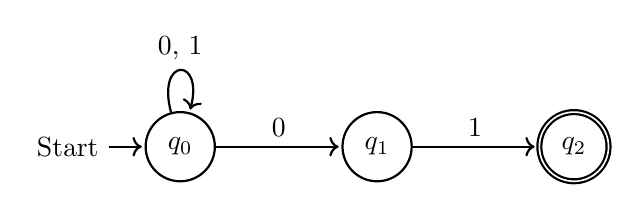
\begin{tikzpicture}[shorten >=1pt,node distance=2.5cm,on grid,auto, thick]
       \node[state,initial,initial text=Start] (q0) {$q_0$};
       \node[state] (q1) [right=of q0] {$q_1$};
       \node[state,accepting] (q2) [right=of q1] {$q_2$};

       \path[->] 
       (q0) edge [loop above] node {0, 1} (q0)
            edge node {0} (q1)
       (q1) edge node {1} (q2);
    \end{tikzpicture}
    \caption{NFA Asal: Pola Akhiran "01"}
\end{figure}

Langkah pertama yang harus banget dilakukan adalah bikin \textbf{Tabel Transisi NFA}-nya dulu biar gampang diliat:

\begin{table}[h]
\centering
\begin{tabular}{@{}ccc@{}}
\toprule
\textbf{State NFA} & \textbf{Input 0} & \textbf{Input 1} \\ \midrule
$\rightarrow q_0$ & $\{q_0, q_1\}$ & $\{q_0\}$ \\
$q_1$ & $\emptyset$ & $\{q_2\}$ \\
$*q_2$ & $\emptyset$ & $\emptyset$ \\ \bottomrule
\end{tabular}
\end{table}

\subsection{Proses Eksekusi Konversi}
Kita mulai bikin state DFA dari state awal NFA. Biar nggak bingung, state DFA kita kasih nama pakai huruf besar ($A, B, C$, dst).

\textbf{Langkah 1: Tentukan Start State DFA} \\
Start state DFA kita namakan state $A$. Isinya adalah start state NFA yaitu $q_0$.
\[ A = \{q_0\} \]

\textbf{Langkah 2: Telusuri Transisi dari State A} \\
Sekarang kita cek, kalau dari $A$ dikasih input '0' dan '1', tujuannya ke mana aja berdasarkan tabel NFA di atas?
\begin{itemize}
    \item $A$ baca '0' $\Rightarrow$ lihat baris $q_0$ kolom 0 $\Rightarrow$ Hasilnya $\{q_0, q_1\}$. Ini kan himpunan baru nih, kita kasih nama state \textbf{$B$}.
    \item $A$ baca '1' $\Rightarrow$ lihat baris $q_0$ kolom 1 $\Rightarrow$ Hasilnya $\{q_0\}$. Ini kan si state \textbf{$A$} itu sendiri.
\end{itemize}

\textbf{Langkah 3: Telusuri State Baru (State B)} \\
State $B = \{q_0, q_1\}$. Cara ngecek transisinya adalah dengan menggabungkan hasil transisi $q_0$ dan $q_1$.
\begin{itemize}
    \item $B$ baca '0' $\Rightarrow$ transisi $q_0$ baca '0' \textbf{digabung} transisi $q_1$ baca '0'. \\
    Hasilnya: $\{q_0, q_1\} \cup \emptyset = \{q_0, q_1\}$. Loh, balik lagi ke state \textbf{$B$}.
    \item $B$ baca '1' $\Rightarrow$ transisi $q_0$ baca '1' \textbf{digabung} transisi $q_1$ baca '1'. \\
    Hasilnya: $\{q_0\} \cup \{q_2\} = \{q_0, q_2\}$. Ini himpunan baru lagi! Kita kasih nama state \textbf{$C$}.
\end{itemize}

\textbf{Langkah 4: Telusuri State Baru (State C)} \\
State $C = \{q_0, q_2\}$. 
\begin{itemize}
    \item $C$ baca '0' $\Rightarrow$ $\{q_0, q_1\} \cup \emptyset = \{q_0, q_1\}$. Balik ke state \textbf{$B$}.
    \item $C$ baca '1' $\Rightarrow$ $\{q_0\} \cup \emptyset = \{q_0\}$. Balik ke state \textbf{$A$}.
\end{itemize}

Karena udah nggak ada state himpunan baru lagi yang muncul, algoritmanya \textbf{selesai}.

\textbf{Langkah 5: Tentukan Final State DFA} \\
Lihat himpunan state A, B, dan C. Himpunan mana yang di dalamnya ada $q_2$ (final state asal NFA)?
\begin{itemize}
    \item $A = \{q_0\}$ (Bukan final)
    \item $B = \{q_0, q_1\}$ (Bukan final)
    \item \textbf{$C = \{q_0, q_2\}$ (Ini FINAL STATE, karena mengandung $q_2$!)}
\end{itemize}

\subsection{Hasil Akhir DFA}
Kalau kita rekap hasil corat-coret di atas, tabel transisi DFA-nya jadi rapi kayak gini:

\begin{table}[h]
\centering
\begin{tabular}{@{}ccll@{}}
\toprule
\textbf{State DFA} & \textbf{Isi Himpunan} & \textbf{Input 0} & \textbf{Input 1} \\ \midrule
$\rightarrow A$ & $\{q_0\}$ & $B$ & $A$ \\
$B$ & $\{q_0, q_1\}$ & $B$ & $C$ \\
$*C$ & $\{q_0, q_2\}$ & $B$ & $A$ \\ \bottomrule
\end{tabular}
\end{table}

Dan diagram mesin DFA barunya bakal kelihatan seperti ini:
\begin{figure}[h]
    \centering
    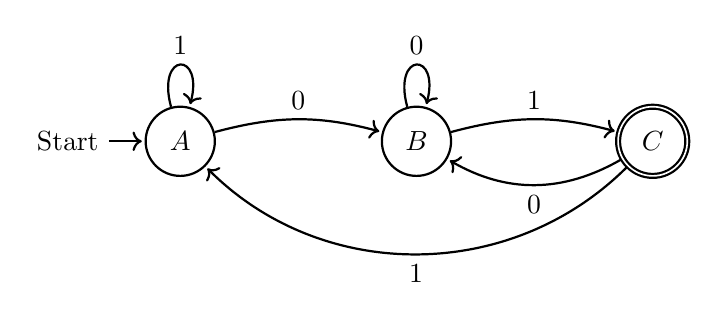
\begin{tikzpicture}[shorten >=1pt,node distance=3cm,on grid,auto, thick]
       \node[state,initial,initial text=Start] (A) {$A$};
       \node[state] (B) [right=of A] {$B$};
       \node[state,accepting] (C) [right=of B] {$C$};

       \path[->] 
       (A) edge [loop above] node {1} (A)
           edge [bend left=15] node {0} (B)
       (B) edge [loop above] node {0} (B)
           edge [bend left=15] node {1} (C)
       (C) edge [bend left=30] node {0} (B)
           edge [bend left=45] node {1} (A);
    \end{tikzpicture}
    \caption{DFA Hasil Konversi (Setara dengan NFA Asal)}
\end{figure}

Gampang, kan? Cuma modal himpunan sama teliti aja baca tabel asalnya.

\newpage
\section{Bumbu Rahasia: $\epsilon$-Closure}

Nah, tadi kan konversi NFA yang polos-polos aja. Gimana kalau NFA-nya pakai transisi jalan tol alias $\epsilon$-transition? Kita butuh jurus tambahan yang namanya \textbf{$\epsilon$-Closure} (ditulis $\epsilon\text{-Cl}$).

\begin{tipbox}
\textbf{Apa itu $\epsilon$-Closure?} \\
$\epsilon$-Closure dari sebuah state adalah \textbf{kumpulan semua state yang bisa didatengin dari state tersebut SECARA GRATIS cuma pakai transisi epsilon ($\epsilon$)}. Jangan lupa, sebuah state itu selalu bisa mendatangi dirinya sendiri secara gratis. Jadi, nama state itu sendiri pasti masuk ke dalam himpunan $\epsilon$-Closure-nya.
\end{tipbox}

Contoh sederhana, kalau kita punya alur $q_1 \xrightarrow{\epsilon} q_2 \xrightarrow{\epsilon} q_3$:
\begin{itemize}
    \item $\epsilon\text{-Cl}(q_1) = \{q_1, q_2, q_3\}$ (Karena dari $q_1$ jalan $\epsilon$ tembus sampai $q_3$)
    \item $\epsilon\text{-Cl}(q_2) = \{q_2, q_3\}$
    \item $\epsilon\text{-Cl}(q_3) = \{q_3\}$ (Nggak ada panah $\epsilon$ keluar dari dia)
\end{itemize}

Setiap kali mesin mau gerak baca satu input karakter, dia harus ngecek $\epsilon$-Closure \textbf{sebelum dan sesudah} pindah.

\newpage
\section{Studi Kasus 2: Epsilon-NFA ke DFA}

Coba kita bedah contoh yang lumayan elegan ini. Kita mau bikin DFA dari NFA yang mengenali bahasa $a^* b^* c^*$ (huruf 'a', terus huruf 'b', terus huruf 'c', masing-masing jumlahnya bebas, boleh nol). Alfabetnya $\Sigma=\{a,b,c\}$.

\begin{figure}[h]
    \centering
    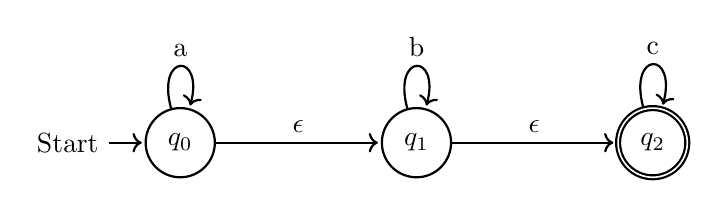
\begin{tikzpicture}[shorten >=1pt,node distance=3cm,on grid,auto, thick]
       \node[state,initial,initial text=Start] (q0) {$q_0$};
       \node[state] (q1) [right=of q0] {$q_1$};
       \node[state,accepting] (q2) [right=of q1] {$q_2$};

       \path[->] 
       (q0) edge [loop above] node {a} (q0)
            edge node {$\epsilon$} (q1)
       (q1) edge [loop above] node {b} (q1)
            edge node {$\epsilon$} (q2)
       (q2) edge [loop above] node {c} (q2);
    \end{tikzpicture}
    \caption{Epsilon-NFA untuk Pola $a^*b^*c^*$}
\end{figure}

\textbf{Langkah 1: Hitung $\epsilon$-Closure Tiap State} \\
Biar enak, kita inventarisir dulu jalan gratis dari tiap state:
\begin{itemize}
    \item $\epsilon\text{-Cl}(q_0) = \{q_0, q_1, q_2\}$ (Tembus dari awal sampai akhir!)
    \item $\epsilon\text{-Cl}(q_1) = \{q_1, q_2\}$
    \item $\epsilon\text{-Cl}(q_2) = \{q_2\}$
\end{itemize}

\textbf{Langkah 2: Tentukan Start State DFA} \\
Beda sama sebelumnya, start state DFA sekarang \textbf{bukan cuma} $\{q_0\}$, melainkan hasil $\epsilon\text{-Cl}(q_0)$. Begitu mesin dinyalain, dia langsung menjalar ke mana-mana.
Kita namain state awal DFA ini $A$.
\[ A = \epsilon\text{-Cl}(q_0) = \{q_0, q_1, q_2\} \]

\textbf{Langkah 3: Cek Transisi dari State A} \\
Rumus kalau mau ngecek transisi di Epsilon-NFA: \\
$\delta_{\text{DFA}}(A, \text{input}) = \epsilon\text{-Cl}( \text{Gabungan pindahan tiap elemen di A} )$

Evaluasi dari $A = \{q_0, q_1, q_2\}$:
\begin{itemize}
    \item \textbf{Input 'a':} \\
    Siapa di dalam $\{q_0, q_1, q_2\}$ yang punya panah 'a'? Cuma $q_0$, tujuannya ke $q_0$.\\
    Kita tutup lagi pakai $\epsilon$-Closure: $\epsilon\text{-Cl}(q_0) = \{q_0, q_1, q_2\}$.\\
    Hasilnya balik lagi ke state \textbf{$A$}.

    \item \textbf{Input 'b':} \\
    Siapa yang punya panah 'b'? Cuma $q_1$, tujuannya ke $q_1$.\\
    Kita tutup pakai $\epsilon$-Closure: $\epsilon\text{-Cl}(q_1) = \{q_1, q_2\}$.\\
    Ini state baru, kita namain \textbf{$B$}.

    \item \textbf{Input 'c':} \\
    Siapa yang punya panah 'c'? Cuma $q_2$, tujuannya ke $q_2$.\\
    Kita tutup pakai $\epsilon$-Closure: $\epsilon\text{-Cl}(q_2) = \{q_2\}$.\\
    Ini state baru juga, kita namain \textbf{$C$}.
\end{itemize}

\textbf{Langkah 4: Telusuri State B = $\{q_1, q_2\}$}
\begin{itemize}
    \item \textbf{Input 'a':} Nggak ada yang punya panah 'a'. Hasilnya Himpunan Kosong $\emptyset$. Kita sebut state ini \textbf{$D$} (Dead State).
    \item \textbf{Input 'b':} Cuma $q_1$ yang punya. Hasilnya $\epsilon\text{-Cl}(q_1) = \{q_1, q_2\}$. Balik ke state \textbf{$B$}.
    \item \textbf{Input 'c':} Cuma $q_2$ yang punya. Hasilnya $\epsilon\text{-Cl}(q_2) = \{q_2\}$. Maju ke state \textbf{$C$}.
\end{itemize}

\textbf{Langkah 5: Telusuri State C = $\{q_2\}$}
\begin{itemize}
    \item \textbf{Input 'a':} Kosong $\Rightarrow D$
    \item \textbf{Input 'b':} Kosong $\Rightarrow D$
    \item \textbf{Input 'c':} Punya panah 'c'. $\epsilon\text{-Cl}(q_2) = \{q_2\}$. Balik ke \textbf{$C$}.
\end{itemize}

\textbf{Langkah 6: Telusuri State D = $\emptyset$}
Karena Dead State, dikasih input 'a', 'b', atau 'c' bakal tetep di \textbf{$D$}.

\textbf{Langkah 7: Tentukan Final State DFA} \\
Syaratnya, himpunan yang memuat $q_2$ adalah Final State.
\begin{itemize}
    \item $A = \{q_0, q_1, \textbf{q\_2}\}$ $\Rightarrow$ \textbf{FINAL}
    \item $B = \{q_1, \textbf{q\_2}\}$ $\Rightarrow$ \textbf{FINAL}
    \item $C = \{\textbf{q\_2}\}$ $\Rightarrow$ \textbf{FINAL}
\end{itemize}
Wow! State A, B, dan C semuanya jadi Final State.

\subsection{Hasil DFA Epsilon-NFA}
Hasil akhir diagram transisinya bakal jadi seperti ini:
\begin{figure}[h]
    \centering
    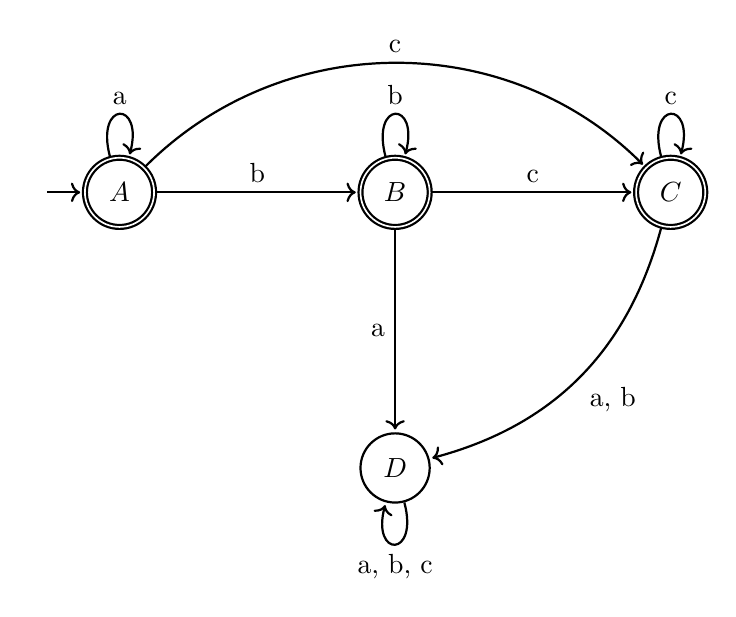
\begin{tikzpicture}[shorten >=1pt,node distance=3.5cm,on grid,auto, thick]
       \node[state,initial,initial text=,accepting] (A) {$A$};
       \node[state,accepting] (B) [right=of A] {$B$};
       \node[state,accepting] (C) [right=of B] {$C$};
       \node[state] (D) [below=of B] {$D$};

       \path[->] 
       (A) edge [loop above] node {a} (A)
           edge node {b} (B)
           edge [bend left=45] node {c} (C)
       (B) edge node [swap] {a} (D)
           edge [loop above] node {b} (B)
           edge node {c} (C)
       (C) edge [bend left] node {a, b} (D)
           edge [loop above] node {c} (C)
       (D) edge [loop below] node {a, b, c} (D);
    \end{tikzpicture}
    \caption{DFA Hasil Konversi Epsilon-NFA $a^*b^*c^*$}
\end{figure}

Dari sini kita bisa lihat betapa rapinya DFA menutupi kerumitan jalan gaib si $\epsilon$. Mesin DFA di atas serba pasti, nggak ada jalan nyabang, dan bisa langsung di-coding ke dalam bahasa pemrograman betulan!

\end{document}